
\begin{frame}[shrink=10, label=completed]
    % \frametitle{Summary of Work Completed}
    \frametitle{My Research}
    \vspace{0.25cm}
    {\footnotesize \setbeamertemplate{itemize item}{$\bullet$}
    \begin{columns}
        \begin{column}{0.8\textwidth}
            Develop and deploy the \hl{\textbf{Zephyr meteor radar network}}
            \begin{itemize} \scriptsize
                \item Hardware, software, testing, and deployments
                \item [{\scriptsize\alert{\(\blacktriangleright\)}}] \alert{Innovating instrumentation}
            \end{itemize}

            \uncover<2->{GNSS-like \hl{\textbf{time-of-flight position solution}} for better locating meteors
            \begin{itemize} \scriptsize
                \item Eliminates calibration, careful array placements
                \item Expected to match or exceed interferometry's precision
                \item Provides easily derived positional uncertainties
                \item[{\scriptsize\alert{\(\blacktriangleright\)}}] \alert{Towards better quantified uncertainties, easier wide-scale deployments}
            \end{itemize} }

            \uncover<3->{Investigating the \hl{\textbf{direction of atmospheric tides}}
            \begin{itemize} \scriptsize
                \item Dividing field-of-view into three virtual instruments 
                \item Analyze spatial progression across windows
                \item Investigated five years of data from the McMurdo meteor radar
                \item[{\scriptsize\alert{\(\blacktriangleright\)}}] \alert{Towards better information extraction} 
            \end{itemize} }

            \uncover<4->{\hl{\textbf{Simulating meteor radar networks}} to understand system performance
            \begin{itemize} \scriptsize
                \item (1) Generate population of meteors, (2) simulate scattering, (3) investigate
                \item Validated by simulating a real system
                \item[{\scriptsize\alert{\(\blacktriangleright\)}}] \alert{Understanding performance supports better science} 
            \end{itemize}}


        \end{column}
        \begin{column}{0.3\textwidth}
            \centering 
            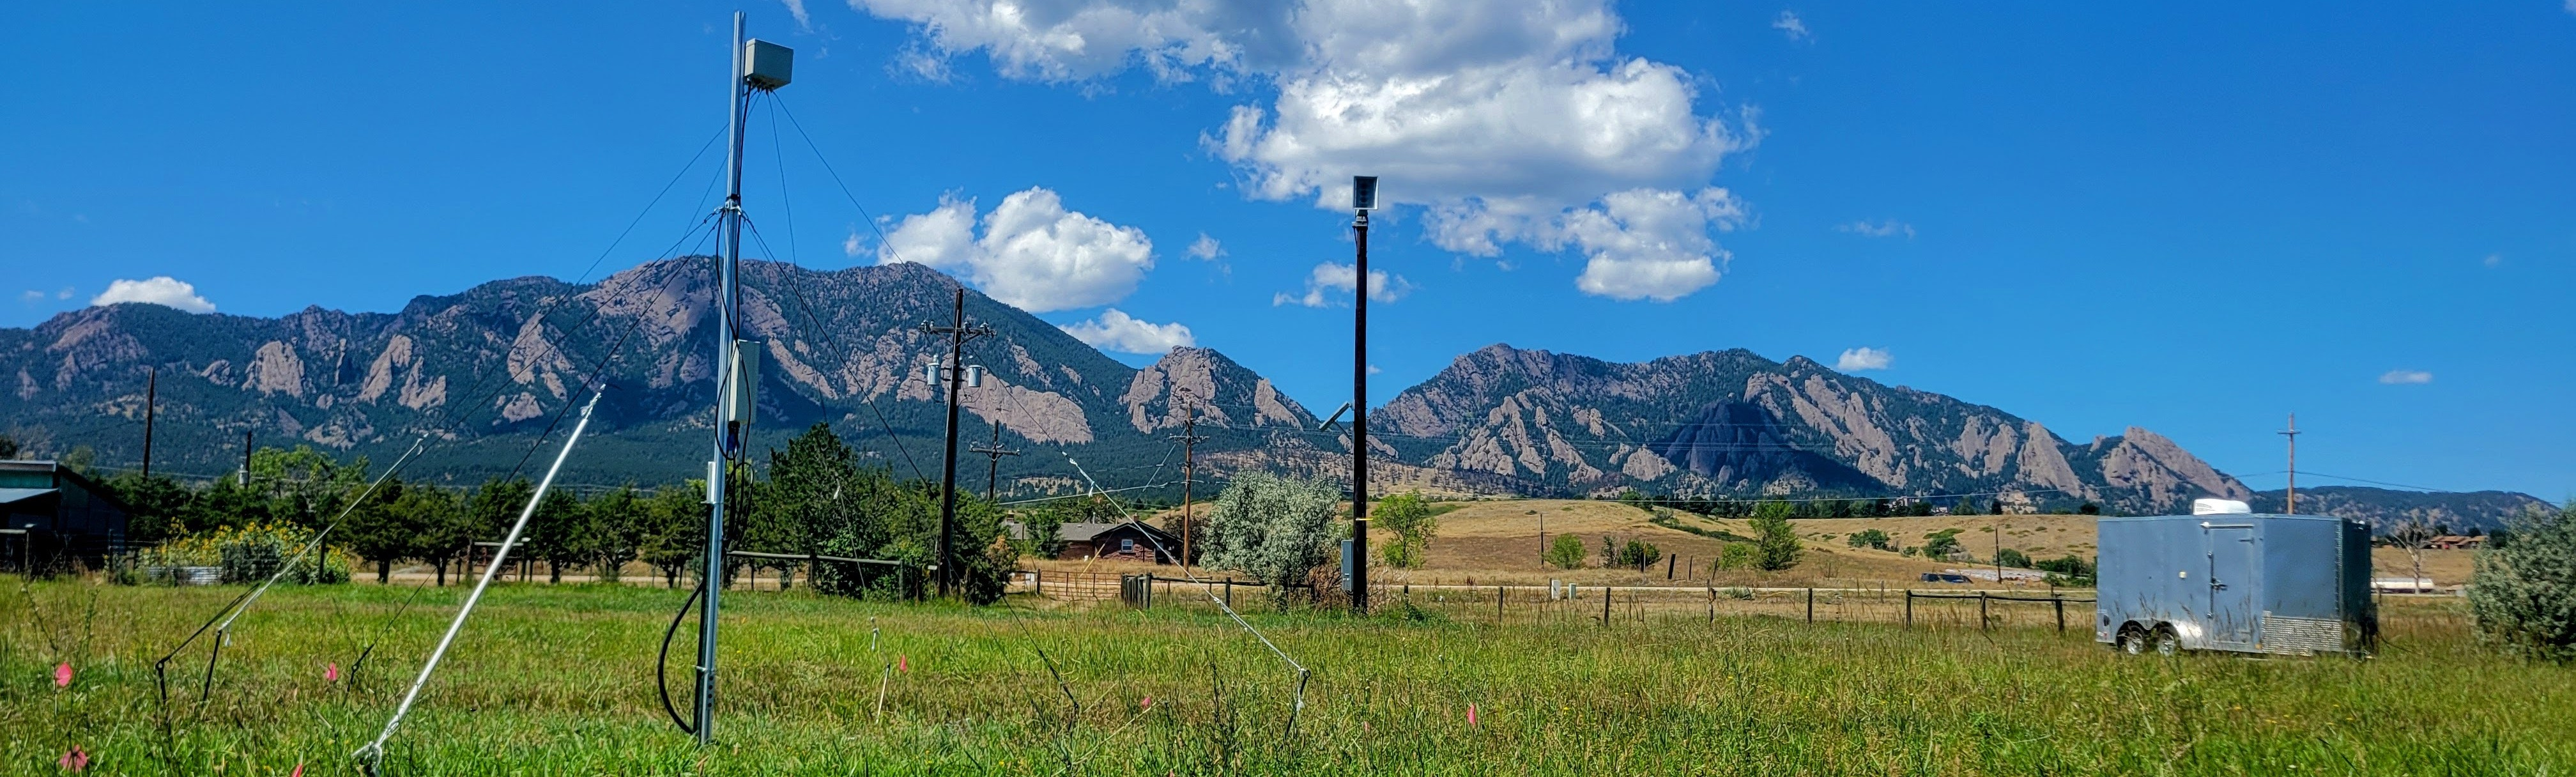
\includegraphics[width=\linewidth]{img/zephyr.jpg}
            \uncovergraphics<2->[height=2cm]{img/0.6km_performance.pdf}
            \uncovergraphics<3->[height=2cm]{img/novel_binning.pdf}
            \uncovergraphics<4->[height=2cm]{img/GIP_expect.pdf}
            \uncovergraphics<4->[height=2cm]{img/simulated_heatmap_200km.pdf}
        \end{column}
    \end{columns}}
\end{frame}